%%%%%%%%%%%%%%%%%%%%%%%%%%%%%%%%%%%%%%%%%%%%%%%%%%%%%%%%%%%%%%%%%%%%%%%%%%%%%%%
\section{A Single-Step Framework for MGXS Generation}
\label{sec:single-step}
%%%%%%%%%%%%%%%%%%%%%%%%%%%%%%%%%%%%%%%%%%%%%%%%%%%%%%%%%%%%%%%%%%%%%%%%%%%%%%%

In general, MGXS generation schemes use a multi-step approach to decouple the energy, angular and spatial dimensions of the transport equation. The multi-step approach typically applies high-fidelity models of the energy self-shielding physics to low-fidelity geometric models of unique core components as illustrated in \autoref{fig:multi-step-framework}. The multi-step approach uses a combination of models of varying complexity to optimize overall simulation speed with accuracy. However, this is often done at the expense of generality. For example, multi-step MGXS generation schemes do not typically model inter-assembly physics or the effect of reflectors and other core heterogeneities on the spatial distribution of the flux. Instead, geometric heuristics such as Dancoff factors are often used to embed spatial self-shielding effects in MGXS for similarly shielded spatial zones (\textit{e.g.}, fuel pins with similar neighboring pins). The approximations to the energy and spatial variation of the flux introduce approximation error in full-core calculations and limit the core design parameter space for which multi-step schemes may be applied. 

\begin{figure}[h!]
\centering
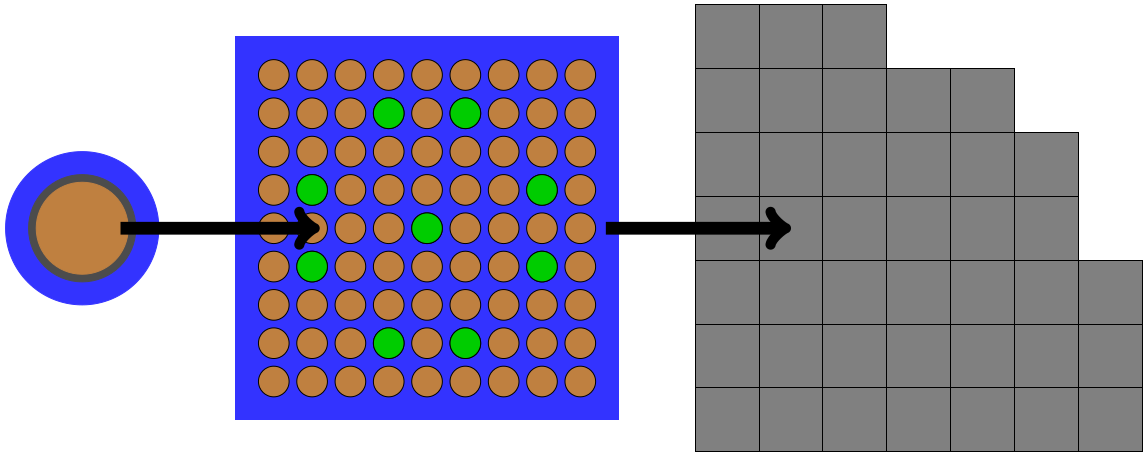
\includegraphics[width=\linewidth]{figures/multi-step-flow-chart}
\caption{The multi-step approach typically used for deterministic reactor physics calculations \citep{gibson2016thesis}.}
\label{fig:multi-step-framework}
\end{figure}

This paper employs Monte Carlo methods to generate MGXS since they present a natural approach to replace engineering prescriptions to approximate the flux with a stochastic approximation of the exact flux. However, MC-based MGXS generation methods to date have retained the multi-step geometric framework to tabulate MGXS for individual reactor components -- such as infinite fuel pins and/or assemblies -- for subsequent use in full-core multi-group calculations. Although the use of MC within a multi-step framework eliminates the need to approximate the flux in energy, it does not account for spatial self-shielding effects throughout a reactor core. 

This paper abandons the multi-step approach in favor of a single-step framework that uses MC eigenvalue simulations of the complete heterogeneous geometry to simultaneously account for all energy and spatial effects in a single step. The single-step framework may be impractical for MGXS generation for industrial applications since it is constrained by the slow convergence rate of Monte Carlo tallies. Nevertheless, it allows for the rigorous quantification of approximation errors due to spatial self-shielding models used to generate MGXS, which is the focal point of this paper.
